\subsection{Generisch}

\begin{frame}{Ganz Generisch}
	\begin{itemize}[<+->]
		\item Eigentlich haben wir kein Universum, keine Prädikate und keine Funktionen vorgegeben
		\item Gegeben ist nur eine Prädikatenlogische Formel
		\item Wir müssen bestimmen ob diese irgendwie erfüllbar ist
	\end{itemize}
\end{frame}

\begin{frame}{Beispiel}
	\note{Dieses Beispiel erweitert das Universum immer um ein Element und geht ein paar Möglichkeiten durch das Prädikat anzuwenden.
		Ein Pfeil von Knoten $X$ auf $Y$ im Graphen bedeutet, dass das $P(X, Y)$ wahr ist, ein fehlender Pfeil, dasss es falsch ist.
		\par
		Dieses Beispiel wurde aus der Ergänzung für Theo II 2018 von Carlos Carmino übernommen
		https://fmi.uni-stuttgart.de/ti/teaching/s18/eti2/ (Termin 1)
	}
	\begin{center}
		\begin{tikzpicture}[overlay]
			\only<4,8|handout:3,4>{
				\node[] (a) at (-2cm, 0){\textcolor{green}{JA}};
				\draw[->] (a) to (-2.4cm, -1cm);
			}
			\only<3,5,6,7|handout:2>{
				\node[] (a) at (-2cm, 0){\textcolor{red}{NEIN}};
				\draw[->] (a) to (-2.4cm, -1cm);
			}

			\only<3,5,6,7,8|handout:2,4>{
				\node[] (b) at (0,0) {\textcolor{green}{JA}};
				\draw[->] (b) to (0, -1cm);
			}
			\only<4|handout:3>{
				\node[] (b) at (0,0) {\textcolor{red}{NEIN}};
				\draw[->] (b) to (0, -1cm);
			}

			\only<3,5,6,7,8|handout:2,4>{
				\node[] (c) at (2cm, 0) {\textcolor{green}{JA}};
				\draw[->] (c) to (2.4cm, -1cm);
			}
			\only<4|handout:3>{
				\node[] (c) at (2cm, 0) {\textcolor{red}{NEIN}};
				\draw[->] (c) to (2.4cm, -1cm);
			}
		\end{tikzpicture}
	\end{center}

	$$
		(\forall X \exists Y: P(X,Y)) \wedge (\forall X: \lnot P(X,X)) \wedge (\exists X \forall Y : \lnot P(Y,X))
	$$

	\begin{center}
		\begin{tikzpicture}[
				base/.style={draw, circle, minimum size = .3cm}
			]
			\only<2-|handout:2->{\node[base] (n0) at (0,0){0};}
			\only<4|handout:3>{\draw[thick,->] (n0.90) arc (0:270:3mm);}

			\only<5-|handout:4->{\node[base, below left = of n0] (n1) {1};}

			\only<7-|handout:4->{\node[base, below right = of n0] (n2) {2};}


			\only<6,7,8|handout:4->{\draw[thick,->] (n0) to (n1);}
			\only<7,8|handout:4->{\draw[thick,->, bend right] (n1) to (n0);}
			\only<8|handout:4->{\draw[thick,->, bend right] (n2) to (n0);}
		\end{tikzpicture}

		%

		\only<1|handout:1>{$U= \emptyset$ müssen wir nicht testen, da das Universum nicht leer sein darf.\\}
		\only<2-4|handout:2-3>{Was ist mit dem Universum, das ein Element hat. Nennen wir das Element mal $0$\\}
		\only<5-6|handout:0>{Lasst es uns mal mit $U= \{0,1\}$ probieren\\}
		\only<7-|handout:4>{Lasst es uns mal mit $U= \{0,1,2\}$ probieren\\}
		\only<1|handout:1>{\vfill \tiny Dieses Beispiel wurde \hyperref{https://fmi.uni-stuttgart.de/ti/teaching/s18/eti2/}{}{}{aus der Ergänzung für Theo II 2018 von Carlos Carmino übernommen}.}
	\end{center}

\end{frame}

\begin{frame}{Formal aufschreiben}
	\alert{Achtung:} Wir müssen das Ergebnis formal aufschreiben!

	\begin{align*}
		U                                   & = \{0,1,2\}                                                      \\
		I(P)                                & = \{(0,1), (1,0), (2,1)\}                                        \\
		\onslide<3->{\textcolor{gray}{I(f)} & = \textcolor{gray}{\{0 \mapsto 1, 1 \mapsto 2, 2 \mapsto 0\} } } \\
		\onslide<4->{\textcolor{gray}{I(a)} & \textcolor{gray}{= 0}}
	\end{align*}

	\begin{tikzpicture}[overlay]
		\only<2>{
			\node[] (a) at (7cm,3.5cm) {Das Universum};
			\node[] (b) at (6.4,0.25) {alle Kombinationen für die das Prädikat zu einer wahren Aussage wird};
			\draw[->] (a) to (5.62cm, 2.9cm);
			\draw[->] (b) to (5.3cm, 2cm);
		}
		\only{
			\node[] (b) at (5.5,-1) {Wenn eine Funktion enthalten wäre, wird diese so angegeben};
			%\node[] at (5,-.9) {(Haben wir im Beispiel nicht)};
			\draw[->] (b) to (5cm, 1.5cm);
		}<3>
		\only{
			\node[] (b) at (3.5,-.4) {Wenn eine Konstante enthalten wäre, wird sie so angegeben};
			%\node[] at (5,-.9) {(Haben wir im Beispiel nicht)};
			\draw[->] (b) to (4.3cm, .8cm);
		}<4>
	\end{tikzpicture}


\end{frame}

{\setbeamercolor{palette primary}{bg=ExColor}
\begin{frame}{Denkpause}
	Finde Interpretationen, für die die Aussagen stimmen
	\metroset{block=fill}
	\begin{block}{Normal}
		\begin{itemize}
			\item $\forall x: {P_1(x,f_1(x))}$
			\item $\forall x\ \forall y : P_2(x,y)\land \forall x : \lnot P_2(a_2,x)$ mit $a_2$ Konstante
			\item $\forall x : \left(P_{3a}(x,f_3(x))\land P_{3b}(f_3(x),x)\right)$ mit $U=\mathbb{N}$ %Lösung: f: Nachfolge, P: <, Q: >
		\end{itemize}
	\end{block}
	\begin{block}{Schwer}
		\begin{itemize}
			\item $\cleft[cyan](
				      \forall x\ \forall y\ \forall z :
				      \cleft[green](
				      P_4(x,y) \land P_4(y,z)
				      \cright[green])
				      \implies P_4(x,z)
				      \cright[cyan])
				      \land
				      \cleft[cyan](
				      \forall x\ \forall y : P_4(x,y) \implies P_4(y,x)
				      \cright[cyan])
				      \land
				      \cleft[cyan](
				      \forall x : \lnot P_4(a_4, x) \land \lnot P_4(x, a_4)
				      \cright[cyan])$
			      mit $a_4$ Konstante
			\item $\cleft[cyan](
				      \forall x\ \exists\ y \forall\ z \in U\setminus\{y\} : P_5(x,y)\land\lnot P_5(x,z)
				      \cright[cyan])
				      \land
				      \cleft[cyan](
				      \forall x,y\ \exists z_0,\dots,z_n : P_5(x,z_0) \land \cleft[green](
				      \bigwedge_{i=0}^{n-1} P_5(z_i,z_{i+1})
				      \cright[green])
				      \land P_5(z_n,y)
				      \cright[cyan])$
		\end{itemize}
	\end{block}
\end{frame}

\begin{frame}<handout:0>{Lösungen}
	\textit{Je Beispiele, es gibt weitere Lösungen}
	\begin{itemize}[<+- | alert@+>]
		\item $U=\{0\}$ \only<1>{\\}\only<2->{; }
		      $I_1(P_1) = \{(0,0)\}$ \only<1>{\\}
		      $I_2(f_1) = \{0\mapsto 0\}$
		\item Es gibt keine Interpretation, die die Aussage erfüllt, da $P_2$ für jede $x,y$ Kombination wahr sein soll aber trotzdem Kombinationen mit einem $a_2$ geben soll für die $P_2$ falsch ist.
		\item $U=\mathbb{N}$ (geg.) \only<3>{\\}\only<4->{; }
		      $I_3(P_{3a}) = \{(a,b)\mid a < b\}$ \only<3>{\\}\only<4->{; }
		      $I_3(P_{3b}) = \{(a,b)\mid a > b\}$ \only<3>{\\}\only<4->{; }
		      $I_3(f_3) = \{n\mapsto n+1 \mid n\in \mathbb{N}\}$
		\item $U=\text{Menge aller Aussagen}$ \only<4>{\\}\only<5->{; }
		      $I(P_4)=\{(a,b)\mid a \land b$ ist wahr$\}$ \only<4>{\\}\only<5->{; }
		      $I(a_4): \text{falsch}$
	\end{itemize}

\end{frame}

\begin{frame}<handout:0>{Lösungen}
	\textit{Je Beispiele, es gibt weitere Lösungen}
	\par
	\begin{tikzpicture}[
			base/.style={draw, circle, minimum size = .3cm}
		]
		\node[base] (n0) at (0,0){0};
		\node[base, right = of n0] (n1) {1};
		\only<1>{
			\draw[thick,->,bend right] (n0) to (n1);
			\draw[thick,->,bend right] (n1) to (n0);
		}

		\only<2>{
			\node[base, below = of n1] (n2) {2};
			\node[base, below = of n0] (n3) {3};


			\draw[thick,->] (n0) to (n1);
			\draw[thick,->] (n1) to (n2);
			\draw[thick,->] (n2) to (n3);
			\draw[thick,->] (n3) to (n0);
		}
	\end{tikzpicture}
	\par
	\only<1>{
		$U=\{0,1\}$\\
		$I_3(P_5) = \{(0,1),(1,0)\}$
	}
	\only<2>{
		$U=\{0,1,2,3\}$\\
		$I_3(P_5) = \{(0,1),(1,2),(2,3),(3,0)\}$
	}
\end{frame}

\begin{frame}{Zum Knobeln}
	\small
	\metroset{block=fill}
	\begin{block}{}
		\begin{multicols}{2}
			\begin{itemize}
				\item $F_1 = \forall X \exists Y: P_0(X,Y)$
				\item $F_2 = \forall X: \overline{P_0(X,X)}$
				\item $F_3 = \exists Y \forall X: \overline{P_0(X,Y)}$
				\item $F_4 = \forall X: \overline{P_0(X,f(x))}$
				\item {\scriptsize$F_5 = \forall X \forall Y: (P_0(X,f(Y)) \implies P_0(Y,X))$}
				\item $F_6 = P(a, f(f(a)))$
				\item $F_7 = \forall X (\exists Y: P_0(Y,X)\implies P_1(X))$
				\item $F_8 = \overline{P_1(f(f(b)))}$
				\item $F_9 = P(f(c),c)$
			\end{itemize}
		\end{multicols}
		Gib eine Interpretation für $F = \bigwedge_{i=1}^9 F_i$ an
	\end{block}
\end{frame}
}